\chapter {Conclusions and Recommendations}
\label{ch:con}

\section {Conclusions}

This dissertation aims to provide a framework for probable maximum precipitation estimation that is suitable for a changing climate. Over the past decades, traditional estimation approach, mainly moisture maximization that assumes unchanged storm efficiency, has been revisited with high-quality observation and numerical simulations. As summarized in chapter \ref{ch:intro}, these studies identified several flaws in the traditional approach: 1) lack of physics in the key assumptions of maximization procedure; 2) stationarity of traditional PMP versus changing climate; 3) difficulties in the interpretation of PMP results; 4) lack of uncertainty estimation. These studies reveal the risk of traditional PMPs in a changing climate. Thus modernization of PMP estimation method is required.

Earlier investigations suggest that numerical models may be used for PMP modernization. However, up to now, there has been no guidance available on how the models should be reasonably used. In this study, we propose a physics-based approach that allows realistic presentation of the dynamic and thermodynamic effect from the worst meteorological scenarios.

Reliable presentation of extreme precipitation events in numerical models is a prerequisite for the proposed physics-based PMP estimation. Chapter \ref{ch:JHE} established a numerical modeling framework based on one of the most widely used models, the WRF model. This addresses the difficulties in setting up atmospheric numerical models introduced by various parameterization schemes. Taking the epic 2010 Nashville, Tennessee storm as a study case, we examined the performance of various WRF configurations. We found that for extreme precipitation simulation purpose, the combination of medium grid size (5km), Morrison microphysics scheme with Kain-Fritsch cumulus scheme can be taken as a starting point in the model calibration. Through our extended validation, this combination is often among the best model configurations that we tested. Since many atmospheric models share a common collection of parameterization schemes, this recommendation can also be applied to other models.

With such a modeling framework, it is now possible to simulate the extreme events since the 1850s. However, it remains unknown how old storms we can now reliably reconstruct. Chapter \ref{ch:EF} examined our capability of reconstructing extreme precipitation events of various types and locations across the US since the 1900s. Though we started with the optimal framework as concluded in chapter \ref{ch:JHE}, various options were still tested so these old events can be reconstructed as best as we could. We found that with currently available model input (initial/boundary conditions), only those extreme events after the 1940s can be reliably constructed. Therefore, for model-based PMP estimations, the historical storms we should examine are only those after the 1940s. On the other hand, this study confirms the usability of the optimal model configuration as given in chapter \ref{ch:JHE}.

With model constructions of extreme precipitation events ready, reasonable ways to maximize the storm magnitude can be now considered in the model. Chapter \ref{ch:JHM} outlined the guidance to make a physics-based PMP estimation. Through the statistical analysis of major long-term reanalysis products (NARR and ERA-Interim) across the contiguous US, we found that the extreme 3-day precipitation in the west US is more related to extreme vertical fields, while those extreme events in the east US are more related to extreme moisture availability. Therefore, we recommend that the 3-day PMP estimation in the west US should be done through maximization of vertical wind fields, while PMP in the east US should be estimated by maximizing the moisture availability in the model input. Such geographic patterns are stable in our sensitivity test. Also, the findings are consistent with previous studies using different approaches, indicating the results are robust. More importantly, this study provides a way to analyze the extreme precipitation and derive PMP estimation guidelines in other durations and other regions of the world.

At this point, a physics-based PMP estimation framework has been established. Such physics-based approach can be used to derive ensemble estimation (by involving multiple inputs such as the readily available CMIP5 odel data), which would provide valuable uncertainty estimation. Also, the stationarity concerns in traditional PMP can be overcome by estimating PMPs for different periods. However, it remains to be solved how the new PMP estimation can be connected to traditional PMPs, thus be used to evaluate the safety of existing infrastructures. To be specific, both input data and methods have been improved from traditional to physics-based approach. Therefore, it is necessary to understand the impact of each of these changes. To facilitate the transition from traditional PMP estimation approach to the proposed physics-based approach, in chapter \ref{ch:WRR}, we also proposed a novel hybrid approach to bridge these approaches.

The motivation of this hybrid approach is illustrated in figure \ref{fig:1-1} as part of a stepwise evolution. This helps engineering community to achieve a stepwise adoption of physics-based approach, and understand how the different input data and methods would impact the final PMP estimation. Such hybrid approach can also be used as a starting point of checking the existing infrastructures (which are designed under traditional PMPs) under the projected climate change. Compared with previous studies, this hybrid approach makes the most use of the raw (coarse-resolution) climate model data. Thus the computation burden is reduced to the minimum. Taking the US Pacific Northwest as an example, we showed that climate model data with traditional method produced PMPs that were comparable to traditional approach (i.e., based on ground observation data).

Through this dissertation study, a physics-based PMP estimation framework is established. Our suggestion to engineering communities is that while doing more verification/validation (so more systematic instructions similar to current HMRs can be provided), it is now also possible to use the climate model data to reassess the safety of existing infrastructures and fix them as necessary. For HMR-style universal instructions, the proposed hybrid or physics-based approach can be used to derive PMPs of various durations and watershed sizes. More recommendations are outlined in the next section.


\section {Recommendations}

Through our study, we give out guidelines to make physics-based PMP estimation. However, for these guidelines to become engineering protocol, the following works are still needed:

1. Extensive studies are required that validate these recommendations over the historical storms. This is to convince the engineering communities to adopt these guidelines confidently. There have been a number of more objective-based evaluation metrics proposed by other studies [\textit{Davis et al.}, 2006a, 2006b; \textit{Gilleland et al.}, 2009; \textit{Wernli et al.}, 2008]. Figure \ref{fig:6-1} provides such an example using SAL metrics [\textit{Wernli et al.}, 2008], which produced similar results as in chapter \ref{ch:JHE}.

\begin{figure}[htbp]
	\centering
	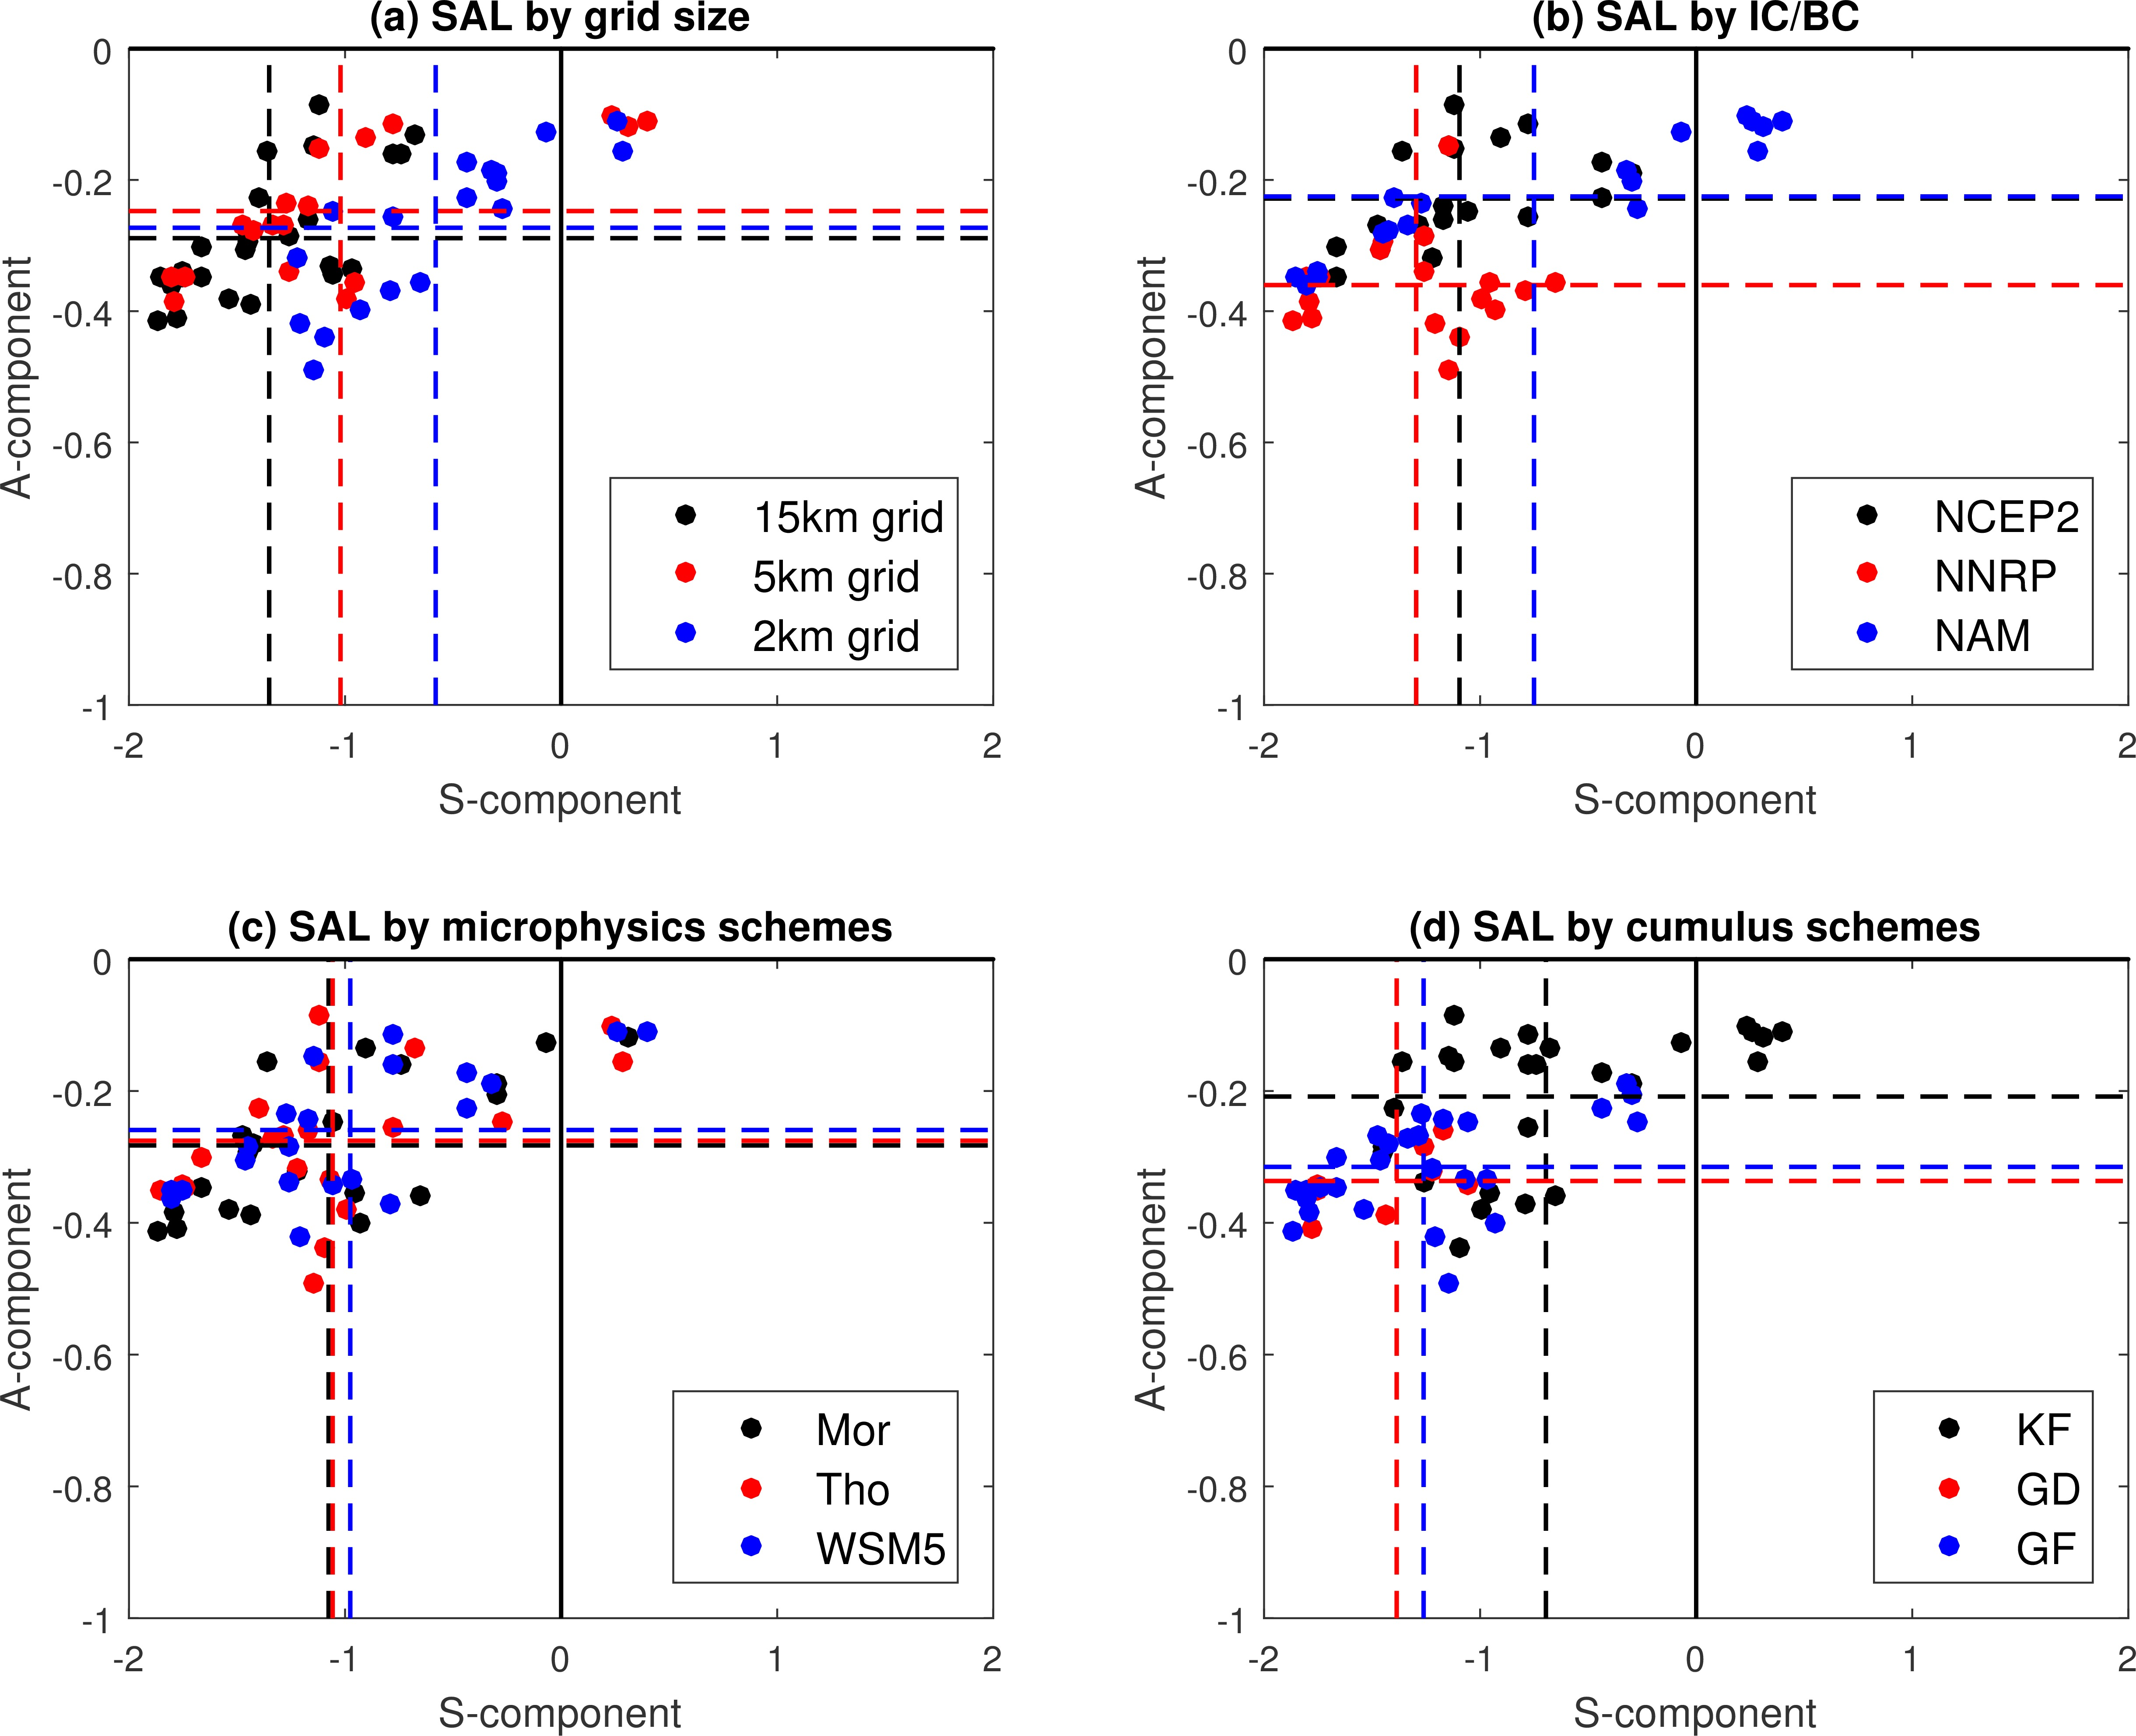
\includegraphics[width=\linewidth]{pics/ch6/fig1.jpg}
	\caption{Evaluation of the WRF simulations in chapter \ref{ch:JHE} using SAL metrics.}
	\label{fig:6-1}
\end{figure}

2. More details on how the model should be run with these guidelines should be investigated. For example, how the simulation boundaries should be defined (right along the watershed boundary v.s. a larger box), how the climatology of vertical wind should be defined for the various precipitation event duration (1-hour to 72-hour), as well as how to systematically set the desired initial/boundary conditions in the model simulation. Eventually, systematic and detailed instructions are required for the engineering practice.

3. In developing the physics-based guidelines, we checked the roles of atmospheric instability, moisture availability, wind fields and temperature profiles in the extreme precipitation duration. It turned out that atmospheric instability and temperature profile do not play a significant role in the extreme precipitation processes across the CONUS. However, this may not be the case for other regions. If any of these factors show significant roles in the storm processes of the other study regions, they should also be analyzed and included in the PMP estimation.

4. So far, all of the above analyses have been done only for the US. With the major reanalysis products available at global scale, it is possible and necessary to conduct such analysis globally. This would reveal the spatial patterns of the relationship between extreme precipitation and environmental conditions at a larger scale. At the same time, such analysis is more useful for the PMP estimation in the regions where long-term ground observation has not been established. Figure \ref{fig:6-2} provides such an example.

With these additional works completed, the proposed physics-based PMP estimation approach would be ready for engineering implementation. With such a fully dynamic method, we can advance our engineering safety design with a more robust basis (i.e., more historical storms that can be taken from atmospheric reanalysis), as well as a more forward-thinking fashion (i.e., designs under a changing climate). Also, we will be ready to explore the various interactions between natural variability, human activities and engineering infrastructure safety in a more coupled and comprehensive way.

\begin{figure}[htbp]
	\centering
	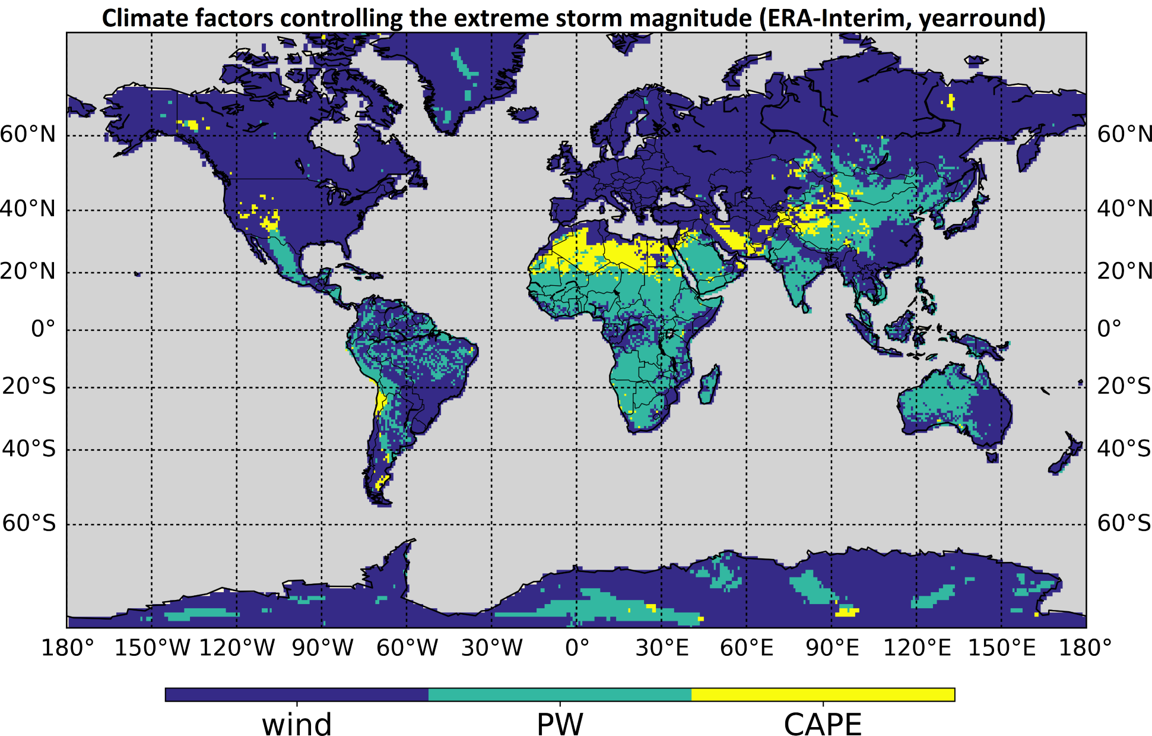
\includegraphics[width=\linewidth]{pics/ch6/fig2.png}
	\caption{A complete transition from traditional approach to physics-based approach of PMP estimation.}
	\label{fig:6-2}
\end{figure}